
\documentclass{beamer}
%\mode<presentation>{\usepackage{beamerthemesplit}}

%\usepackage{beamerthemebars}
\usepackage{amsmath}
\renewcommand{\baselinestretch}{1.2}
\usepackage{cite}
\usepackage{url}
\usepackage{longtable}
%\usepackage[dvips]{graphicx,color}
%\usepackage{makeidx}
\usepackage{nomencl}
\usepackage{amssymb}
%\usepackage{psfig}
%\usepackage{epsfig}
\usepackage{graphicx}
\usepackage{amssymb}
\usepackage{multicol}
\usepackage[bottom]{footmisc}
\usepackage{subfigure}
\usepackage[OT2,OT1]{fontenc}
\newcommand{\imsize}{3in}

\useinnertheme{rounded}
\usecolortheme{whale}
%\usecolortheme{orchid}
\useoutertheme{infolines}
%\useoutertheme{shadow}

%change your title
\title{\textbf{ Stereo Matching Technique using Belief Propagation}}
\subtitle{\textbf{Subject Seminar}}
%\institute{\normalsize{IIT Bombay}}
%\setbeamercolor{title}{fg=white,bg=black}

\begin{document}
\author[Chitra Suresh] {By \\ \vspace{0.05in} \textbf{Chitra Suresh } \\ \vspace{0.01in} {Under the Guidance of} \\ \textbf{Prof.Dr.Kushal.R.Tuckley  }\\
\textcolor{black}{ \\ Department of Electronics Engineering} \\ \textcolor{black}{Ramrao Adik Institute of Technology,\\ Nerul, Navi Mumbai } \\}



\begin{frame}
\frametitle{Introduction}
\begin{itemize}
\item Belief Propagation Techniques uses the degree of a person's belief that an event will occur,rather than the actual probability  of the event will occur.
\item Belief probabilities are  properties of person's belief not the event.
\item Belief Propagation Technique is used to perform inference on graphical  model  such as factor graphs which calculates marginal distribution for each unobserved node
conditional on observed node.
\item Belief Propagation Techniques  are used for performing inference on graphical models such as Bayesian Network and Markov Random Field
\end{itemize}
\end{frame}


%Slide which includes bullated items
\begin{frame}
\frametitle{Analysis of Belief Propagation Techniques}
\textbf{Outline of the seminar}
\begin{enumerate}
\item \textbf{Part 1:{Concepts Related to Belief Propagation Techniques}}
\item \textbf{Part 2:{Applications of Belief Propagation Techniques}}
\end{enumerate}
\end{frame}


%Slide which includes figure
\begin{frame}
\frametitle{\textbf{Outline-Part 1}}
\begin{itemize}
\item \textbf{Probabilistic Formulation}
\item \textbf{Probability Model}
\item \textbf{Probability Language}
\item \textbf{Graphical Representation}
\item \textbf{Bayesian Belief Network}
\item \textbf{Markov Random Field }
\end{itemize}
\end{frame}
\begin{frame}
\frametitle{\textbf{Probabilistic Formulation}}
\begin{itemize}
\item Bayesian Methods provides reasoning about partial beliefs under condition of uncertainty
\item Beliefs measures obey the three basic axioms of probability theory.
\begin{equation}
   0 \leq P(A) \leq 1
\end{equation}

\begin{equation}
    P(Sure Propositions)=1
\end{equation}

\begin{equation}
  P (A    or  B) = P(A)+ P(B)
\end{equation}
 if A and B are mutually exclusive
\end{itemize}
\end{frame}
\begin{frame}
\frametitle{\textbf{Probabilistic Formulation}}
\begin{itemize}
\item The basic expressions in the Bayesian formalism are statement about
\begin{enumerate}
\item Conditional probabilities
\item Product rule is so called \textbf{Chain Rule Formula}.
\end{enumerate}
\item  \begin{equation}
     P(A)= \sum \{P(A\setminus B_i)\times P(B_i)\}
\end{equation}
\item The probability of any event A computed by conditioning it on any set of exhaustive and mutually exclusive events $B_i,i=1,2,......n$
\item This decomposition provides the basics for the hypothetical or assumption based reasoning in the bayesian formalism.
\end{itemize}
\end{frame}
\begin{frame}
\frametitle{\textbf{Probabilistic Formulation:product rule or Chain Rule Formula}}
\begin{itemize}
\item It states that if  a set of n events $(E{_1},E{_2},......E{_n})$
\item probability of joint event $(E_1,E{_2},......E{_n})$ can be written as a product of n conditional probabilities
\item \begin{equation}
    P(E{_1},E{_2},......E{_n})=P(E_{n}|E_{n-1},......E{_2},E{_1})......P(E{_2}|E{_1})P(E{_1})
\end{equation}

\item This product can be derived by repeated application of equation 6 in any convenient order.
\item \begin{equation}
P(A,B)=P(A|B)P(B)
\end{equation}
\end{itemize}
\end{frame}
\begin{frame}
\frametitle{\textbf{Probability Model}}
\begin{itemize}
\item  It is an encoding of the probabilistic information in some domain of interest
\item It is formed sentence,statement or proposition which can be calculated in accordance with axioms of probability theory.
\item These sentences are represented by interrelating random or stochastic variables with in model.
\item The  probability model (M) is defined by the joint probability of all its variables
\item Each variable may take any one of a set of mutually exclusive or collectively
exhaustive states.
\end{itemize}
\end{frame}

\begin{frame}
\frametitle{\textbf{Probability Language}}
\begin{itemize}
\item It is suited to reasoning under uncertainty and provides suitable frame work for processing the uncertainty relationship between variables of a probabilistic model.
\item Through  axiomatic basis and provide a convenient mechanism for presenting uncertain results.
\item The basic four primitives of probability language are
\begin{enumerate}
\item Likelihood
\item Conditioning
\item Relevance
\item Causation
\end{enumerate}
\end{itemize}
\end{frame}


\begin{frame}
\frametitle{\textbf{Probability Language}}
\begin{itemize}
\item \textbf{A likelihood} of event  is measure of  how likely or probable that  event will occur ie.chance of occurrence.
\item \textbf{A conditioning :}An event is conditional when it changes by the knowledge of second event states.
\item \textbf{Relevance:}  Two events are relevance,when common sequences is observed.ie event A and event B are relevant if both are causes of event C.
\item \textbf{Causation} conveys a pattern of dependence between events.
\end{itemize}
\end{frame}

\begin{frame}
\frametitle{\textbf{Graphical Representation}}
\begin{itemize}
\item A probabilistic model is dependency model in which  relationship between each of the variable is captured.
\item Graphs may be used to represent dependency model.Dependency Model M comprising the variables U represented by graph.
\item A graph is denoted by G(V,E) is set of nodes or vertices V connected by the set of arcs or edge E.
\item The set of arc E represents conditional dependencies between these variables.
\item ie.Joint probability function of M is encoded in E,Nodes of the graph corresponds to variables in dependency model
\end{itemize}
\end{frame}
\begin{frame}
\frametitle{\textbf{Graphical Representation}}
\begin{itemize}
\item Graphical representation for probabilistic model are two types
\item \textbf{ Undirected graph and Directed graph.}
\item Undirected graph had no explicit direction,an arc of influence between connected nodes.
\item Examples of undirected graph is Markov Random Fields.
\item In directed graph arcs are either unidirectional or bidirectional directed arc provide the mechanism for representing causation
\item Example for Directed graph is Bayesian network
\end{itemize}
\end{frame}
\begin{frame}
\frametitle{\textbf{Bayesian Belief Network}}
\begin{itemize}
\item The Bayesian Belief Network(BBN) determines the state probabilities of each node or variable from predetermined conditional and prior probabilities.
\item The Direct Acyclic Graph G(U,E)of the probability model M represents probability distribution P(U) ,where U represents set of all variables in M
\item Let X${_1}$,X${_2}$,........X${_n}$ are Variables in probability distribution P(U)
\item Direct Acyclic Graph(DAG) in which minimal set of variables are designed as parent of each variable is X${_i}$ such that
\begin{equation}\label{}
   P(X{_i}/W);   W\in{X{_1},X{_2}.....X{_{i-1}}}
\end{equation}
\item The above equation is BBN of that probability distribution
\end{itemize}
\end{frame}

\begin{frame}
\frametitle{\textbf{Bayesian Belief Network}}
\begin{equation}
    P(a/b)P(b)=P(a,b)
\end{equation}
In real world all events are conditioned by some context C=c
\begin{equation}
    P(a/b,c)P(b/c)=P(a,b/c)
\end{equation}
The Baye's rule also conditioned on
\begin{equation}
 P(b/a,c)={P(a/b,c)P(b/c)} / {P(a/c)}
\end{equation}
\begin{itemize}
  \item P(b/a,c) is posterior probability of b
  \item P(a/b,c) liklihood probability
  \item P(a/c) Normalized factor
  \item P(b/c) Priori probability of b
\end{itemize}
\end{frame}

\begin{frame}
\frametitle{\textbf{Bayesian Belief Network}}
Normalised factor  for continuous and discrete distributions are given by
\begin{equation}\label{}
    \int_{b} P(a/b,c)p(b/c)db
\end{equation}
\begin{equation}
    \sum_{b}P(a/b,c)p(b/c)
\end{equation}
\end{frame}

\begin{frame}
\frametitle{\textbf{Markov Random Field}}
The following points to consider while applying Markov Random Field to the Belief propagation Technique
\begin{itemize}
\item Markov Random Field  expressed in terms of conditional independence of its non neighbors,once values of neighbors  are known.
\item Assigning of weights to the links of the graph must be handled with caution.
\item The weights are to be used translating evidential data in to meaning full probabilistic inferences such probabilistic model is both consistent and complete.
\item Consistency guarantees that,it don't over load the graph with too many parameters.
\end{itemize}
\end{frame}
\begin{frame}
\frametitle{\textbf{Markov  Random Field}}
\begin{itemize}
 \item For unidirected graph G ,nodes are always adjust to each other.
%\begin{equation}
 % P(A)=\sum \{P(A\setminus B_i)\times P(B_i)\}
%\end{equation}$
\item For each group of nodes known as associate ,assign a nonnegative compatibility function $g{_i}$($c{_i}$) ,which measures the relative degree of compatibility associated with each value assignment c${_i}$ to the variable.
\item Form the product $\prod{_i}$ $g{_i}$($c{_i}$) of the compatibility functions over all associates.

\item Normalize the product of all possible value combinations of the variables of the system
\end{itemize}
\end{frame}

\begin{frame}
\frametitle{\textbf{Markov  Random Field}}


\begin{equation}\label{}
    P( x{_i},....,x{_n}) =K\prod_{i}g{_i}(c{_i})
\end{equation}

where
 \begin{equation}\label{}
    K= 1\div[\sum_{x{_1},...x{_n}}\prod_{i}g{_i}(c{_i})]
 \end{equation}
 The normalized product P in equation 13 is a joint distribution that consists of all conditional independencies of graph G.
\end{frame}

\begin{frame}
\frametitle{\textbf{Outline:Part-2}}
\begin{enumerate}
\item Efficient Belief Propagation for Early Vision.
\item Efficient Loopy Belief Propagation using the Four Color Theorem
\item Markov Network-based Unified Classifier for Face Identification
\item Image Completion Using Efficient Belief Propagation Via Priority Scheduling and Dynamic Pruning
\item Low Memory Cost Block-Based Belief Propagation For Stereo Correspondence
\item Task Parallel Implementation of Belief Propagation in Factor Graphs
\item Hardware-Efficient Belief Propagation
\item PatchMatch Belief Propagation for Correspondence Field Estimation
\item Learning continuous time Bayesian network classifiers
\end{enumerate}
\end{frame}



\begin{frame}
\frametitle{\textbf{1.Efficient Belief Propagation for Early Vision}}
\begin{itemize}
\item Early vision problems such as stereo and image restoration
\item Inference algorithms based on graph cuts and belief propagation give accurate results, but  too slow for practical use.
\item Markov random field models are used in this application.
\item In this application  some of the techniques  are used that substantially improve the running time of the loopy belief propagation .

\end{itemize}
\end{frame}

\begin{frame}
\frametitle{\textbf{1.Efficient Belief Propagation for Early Vision}}

\begin{enumerate}
  \item One of the techniques reduces the complexity of the inference algorithm to be linear rather than quadratic by fixing the number of possible labels for each pixel, which is important for problems such as image restoration that have a large label set.
  \item second  technique speeds up and reduces the memory requirements of belief propagation on grid graphs.
  \item  A third technique is a multi-grid method that makes it possible to obtain good results with a small fixed number of message passing iterations, independent of the size of the input images.
\end{enumerate}

\end{frame}

\begin{frame}
\frametitle{\textbf{1.Efficient Belief Propagation for Early Vision}}
\textbf{Results }
\begin{itemize}
\item Taken together these techniques speed up the standard algorithm by several orders of magnitude and results obtained are.
\item The time necessary to compute a single message update from O ($k^2$ ) to O (k), where k is the number of possible labels for each pixel for the max-product formulation ie.linear rather than quadratic is possible.

\end{itemize}
\end{frame}



\begin{frame}
\frametitle{\textbf{2.Efficient Loopy Belief Propagation using the Four Color Theorem}}
\begin{itemize}
\item Recent work on early vision such as image segmentation, image  denoising, stereo matching, and optical flow uses Markov Random Fields.
\item  Although this formulation yields an NP-hard energy minimization problem, good heuristics have been developed based on graph cuts and belief propagation.
\item  Both approaches still require tens of seconds to solve stereo problems on recent PCs. Such running times are impractical for optical flow and many image segmentation and
denoising problems
\end{itemize}
\end{frame}

\begin{frame}
\frametitle{\textbf{2.Efficient Loopy Belief Propagation using the Four Color Theorem}}
\begin{itemize}
\item To reduce the computational complexity of belief propagation  can be achieved by applying  Four Color Theorem (FCT) which  limits  the maximum number of labels in  image segmentation to four.
\item  Four Color Theorem (FCT) states that   when an image seen as a planar graph is segmented into contiguous regions, there
are only four colors to be assigned to each pixel/node for all  other segments to be
surrounded by different colors .
\end{itemize}
\end{frame}

\begin{frame}
\frametitle{\textbf{2.Efficient Loopy Belief Propagation using the Four Color Theorem}}
\begin{itemize}
\item In the case of Belief Propagation (BP), a key reason for its slow performance is that the algorithm complexity is proportional to both the number
of pixels in the image, and the number of labels in the underlying image segmentation
which is typically high. If  limit the number of labels, its speed performance should improve greatly.
\item By modifying the propagation algorithms like can using a low number of placeholder
labels, that can reuse for non-adjacent segments. These placeholder labels
can then be replaced by the full set of actual labels.
\end{itemize}
\end{frame}

\begin{frame}
\frametitle{\textbf{2.Efficient Loopy Belief Propagation using the Four Color Theorem}}
\begin{itemize}
\item Since image segments form a planar graph Four Color Theorem (FCT)can be applied to fix the four placeholder labels
\item A fast segmentation through the placeholder labels and a fine grained labeling through the
actual labels provides a joint optimization process
\item  The computational time is basically dependent on the number
of placeholder rather than actual labels.
\end{itemize}
\end{frame}

\begin{frame}
\frametitle{\textbf{2.Efficient Loopy Belief Propagation using the Four Color Theorem}}
\textbf{Results}
\begin{itemize}
\item Four-Color Theorem (FCT)based on the max-product
belief propagation technique can be used in early computer vision for solving
MRF problems where an energy is to be minimized.
\item The  Methods used can  improve either the
speed for large images and/or large label sets
\item FCT principle is difficult to apply  where label set is discrete in the case for stereo matching and optical flow where the
disparity cost function takes discrete and unrelated values.This causes slower
convergence but FCT methods  can  be used to solve the above mentioned problems.
\end{itemize}
\end{frame}
\begin{frame}
\frametitle{\textbf{3.Markov Network-based Unified Classifier for Face Identification}}
\begin{itemize}
\item It is a one-to-many identification problem  and has many applications such
as searching for similar face images in a database and face tagging in images and videos.
\item Recent successful face recognition methods,classifiers are  used where similar scores are merged with the predefined parameters.
\item The parameter comes from the training database and it is not the best choice when the input image has different conditions.
\item These methods lead to good accuracy in face verification, but there is no specific framework for the one-to-many identification problem.
\end{itemize}
\end{frame}

\begin{frame}
\frametitle{\textbf{3.Markov Network-based Unified Classifier for Face Identification}}
\begin{itemize}
\item In this paper, a novel recognition framework for the one-to-many identification  is designed, and the simple concept is illustrated in Figure 1.
\item The multiple classifiers have complementary characteristics, unify the multiple classifiers based on a Markov network as shown in Figure 2
\end{itemize}
\end{frame}



\begin{frame}
\frametitle{\textbf{3.Markov Network-based Unified Classifier for Face Identification}}
\begin{figure}
  % Requires \usepackage{graphicx}
  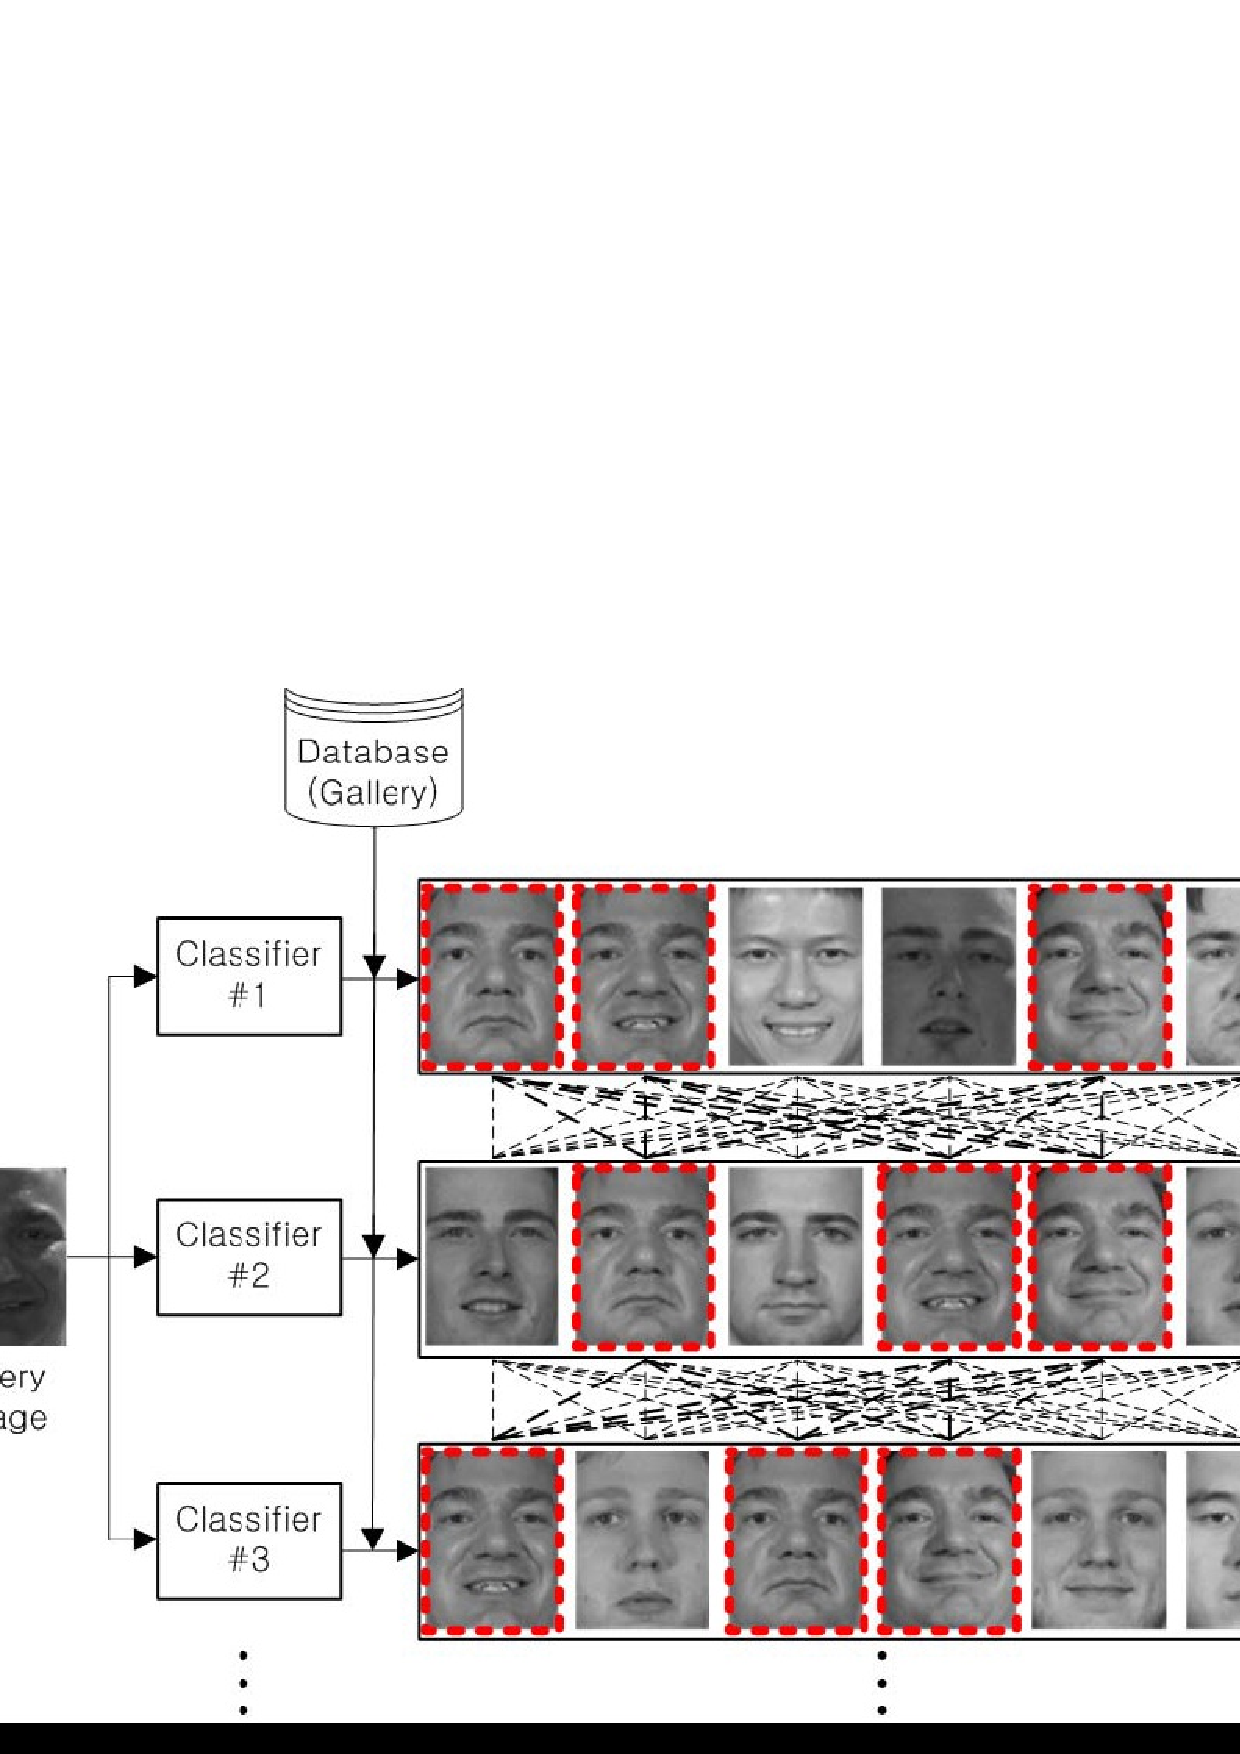
\includegraphics[width=3in]{face.pdf}\\
  \caption{1.One-to-Many identification }
\end{figure}
\end{frame}

\begin{frame}
\frametitle{\textbf{3.Markov Network-based Unified Classifier for Face Identification}}
\begin{figure}
  % Requires \usepackage{graphicx}
  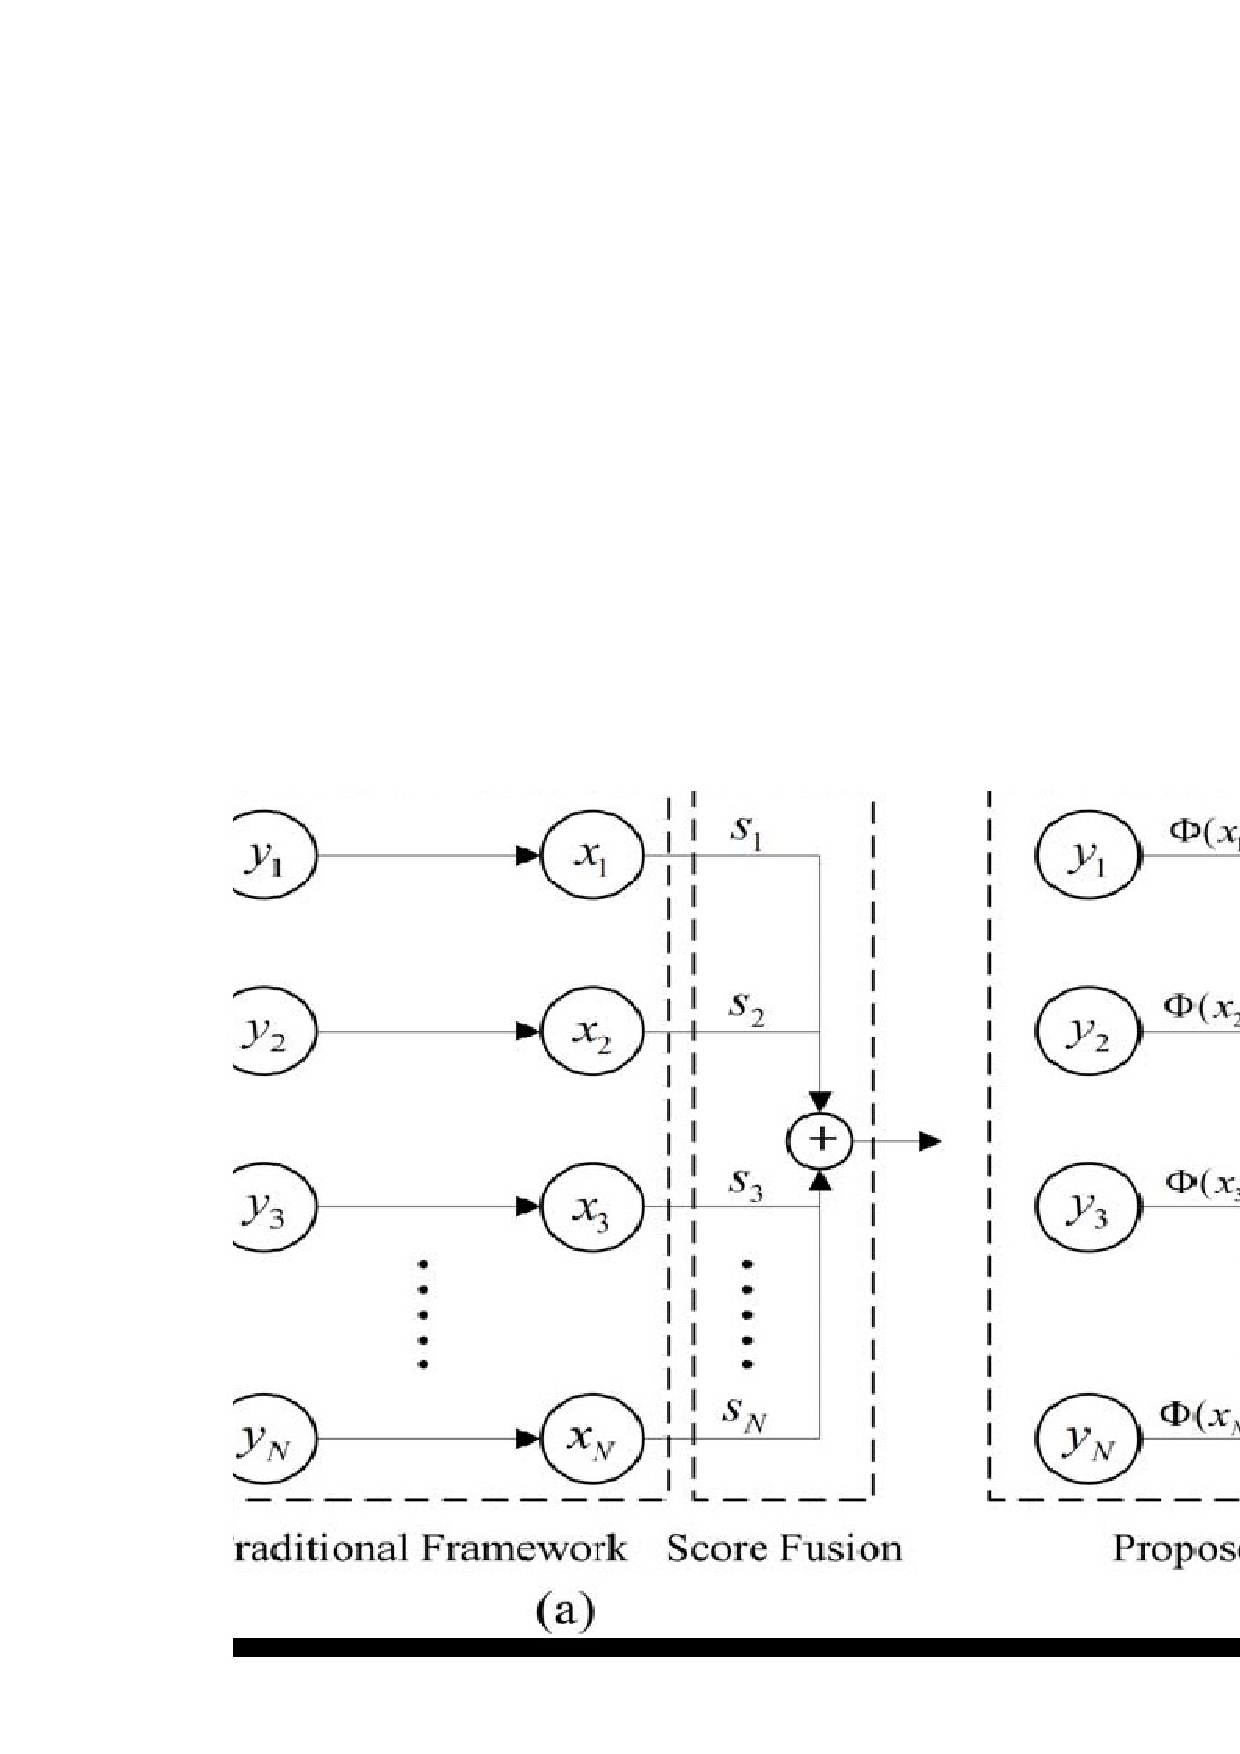
\includegraphics[width=4in]{classifier.pdf}\\
  \caption{2.Traditional and proposed Frame Work}
\end{figure}
\end{frame}

\begin{frame}
\frametitle{\textbf{3.Markov Network-based Unified Classifier for Face Identification}}
\begin{enumerate}
\item steps to find marginal probability by using Markov Fields for classifiers are as follows
\item one node of a Markov network to each classifier,Nodes are connected by lines, which represents the statistical dependencies
\item for an observation node,  extract a feature from a query image using the corresponding classifier.
\item At its paired hidden node, the first retrieve n similar gallery samples from the database.
\end{enumerate}
\end{frame}

\begin{frame}
\frametitle{\textbf{3.Markov Network-based Unified Classifier for Face Identification}}
\begin{enumerate}
\item The multiple classifiers have their own lists of retrieved gallery images, which are not identical in general, thereby complementing the neighbor classifiers.
\item  the hidden nodes are connected by the network lines,
  \item  the relationship between nodes is by selecting similarity scores between the neighbor classifiers,then scores are calculated by concatenating  two gallery features of the neighbor classifiers.


  \item The posterior probability at each hidden node is calculated by the belief-propagation algorithm. Finally, marginal probability for a score value at each classifier is calculated
\end{enumerate}
\end{frame}

\begin{frame}
\frametitle{\textbf{3.Markov Network-based Unified Classifier for Face Identification}}
\begin{itemize}
\item The results obtained are for face recognition particularly for the one-to-many identification task, based on multiple classifiers gallery connected by a Markov network.
\item The Markov network probabilistically models the relationships between a query  images and between neighboring gallery images.
\item The observation-hidden node pair retrieve the  similar gallery images from the database image.
\item The similarities between the retrieved gallery images gives the statistical dependency between the hidden nodes.
\item Hence results obtained can be viewed as clustering-based face recognition.
\end{itemize}
\end{frame}
\begin{frame}
\frametitle{\textbf{4.Image Completion Using Efficient Belief Propagation Via Priority Scheduling and Dynamic Pruning}}

Any algorithm that is designed to solve the image completion problem should have the following characteristics:
\begin{enumerate}
  \item It should be able to successfully complete complex natural images
  \item It should also be able to handle incomplete images with
(possibly) large missing parts
  \item All these should take place in a fully automatic manner, i.e.,
without intervention from the user.
\end{enumerate}
\end{frame}

\begin{frame}
\frametitle{\textbf{4.Image Completion }}
\begin{figure}
  % Requires \usepackage{graphicx}
  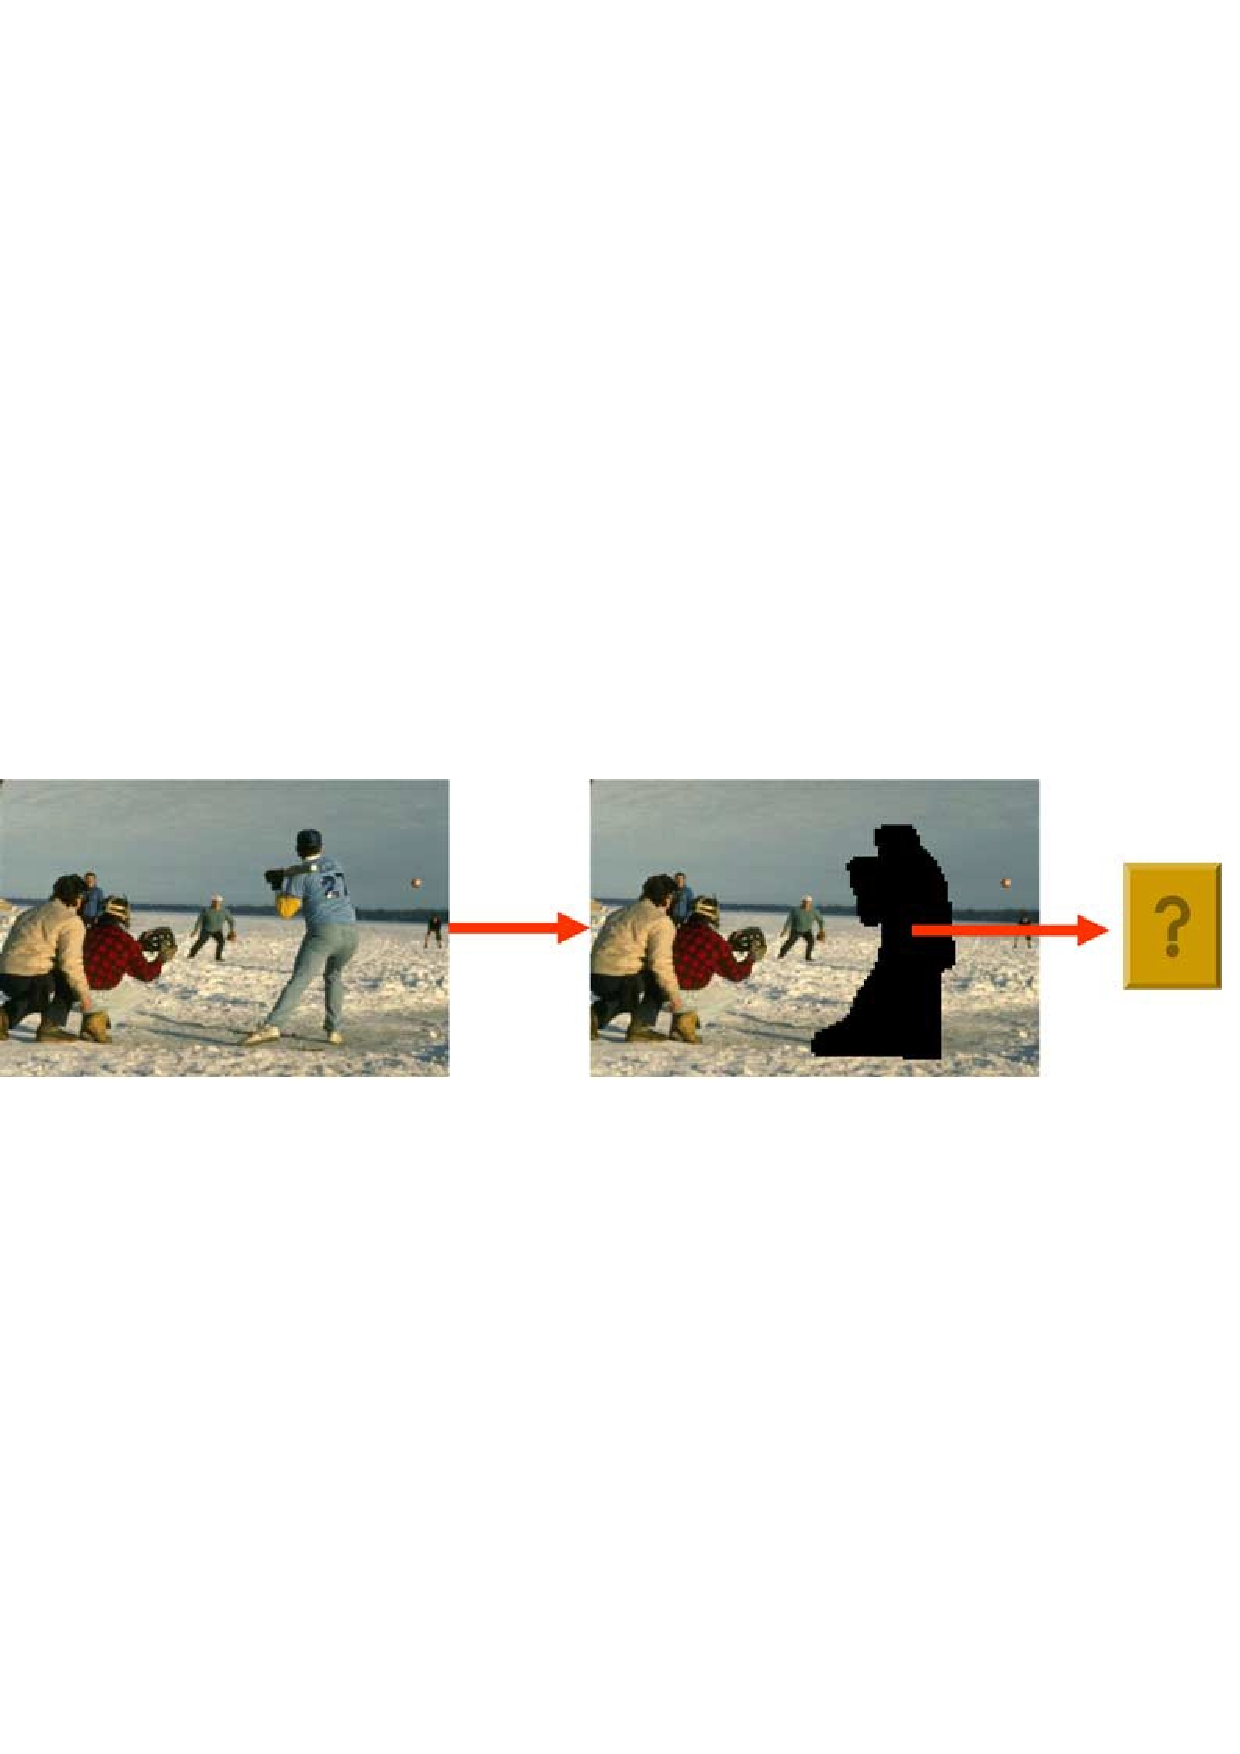
\includegraphics[width=5in]{prune1.pdf}\\
  \caption{Object removal}\label{}
Object removal is just one of the many cases where image completion
needs to be applied.
\end{figure}
\end{frame}

\begin{frame}
\frametitle{\textbf{4.Image Completion Using Efficient Belief Propagation
Via Priority Scheduling and Dynamic Pruning}}
 Three main approaches  for dealing with the image completion problem
\begin{enumerate}
  \item Statistical-based methods
  \item Partial differential equations (PDE)based methods
  \item Exemplar-based methods
\end{enumerate}
\end{frame}
\begin{frame}
\frametitle{\textbf{4.Image Completion Using Efficient Belief Propagation
Via Priority Scheduling and Dynamic Pruning}}
\begin{figure}
  % Requires \usepackage{graphicx}
  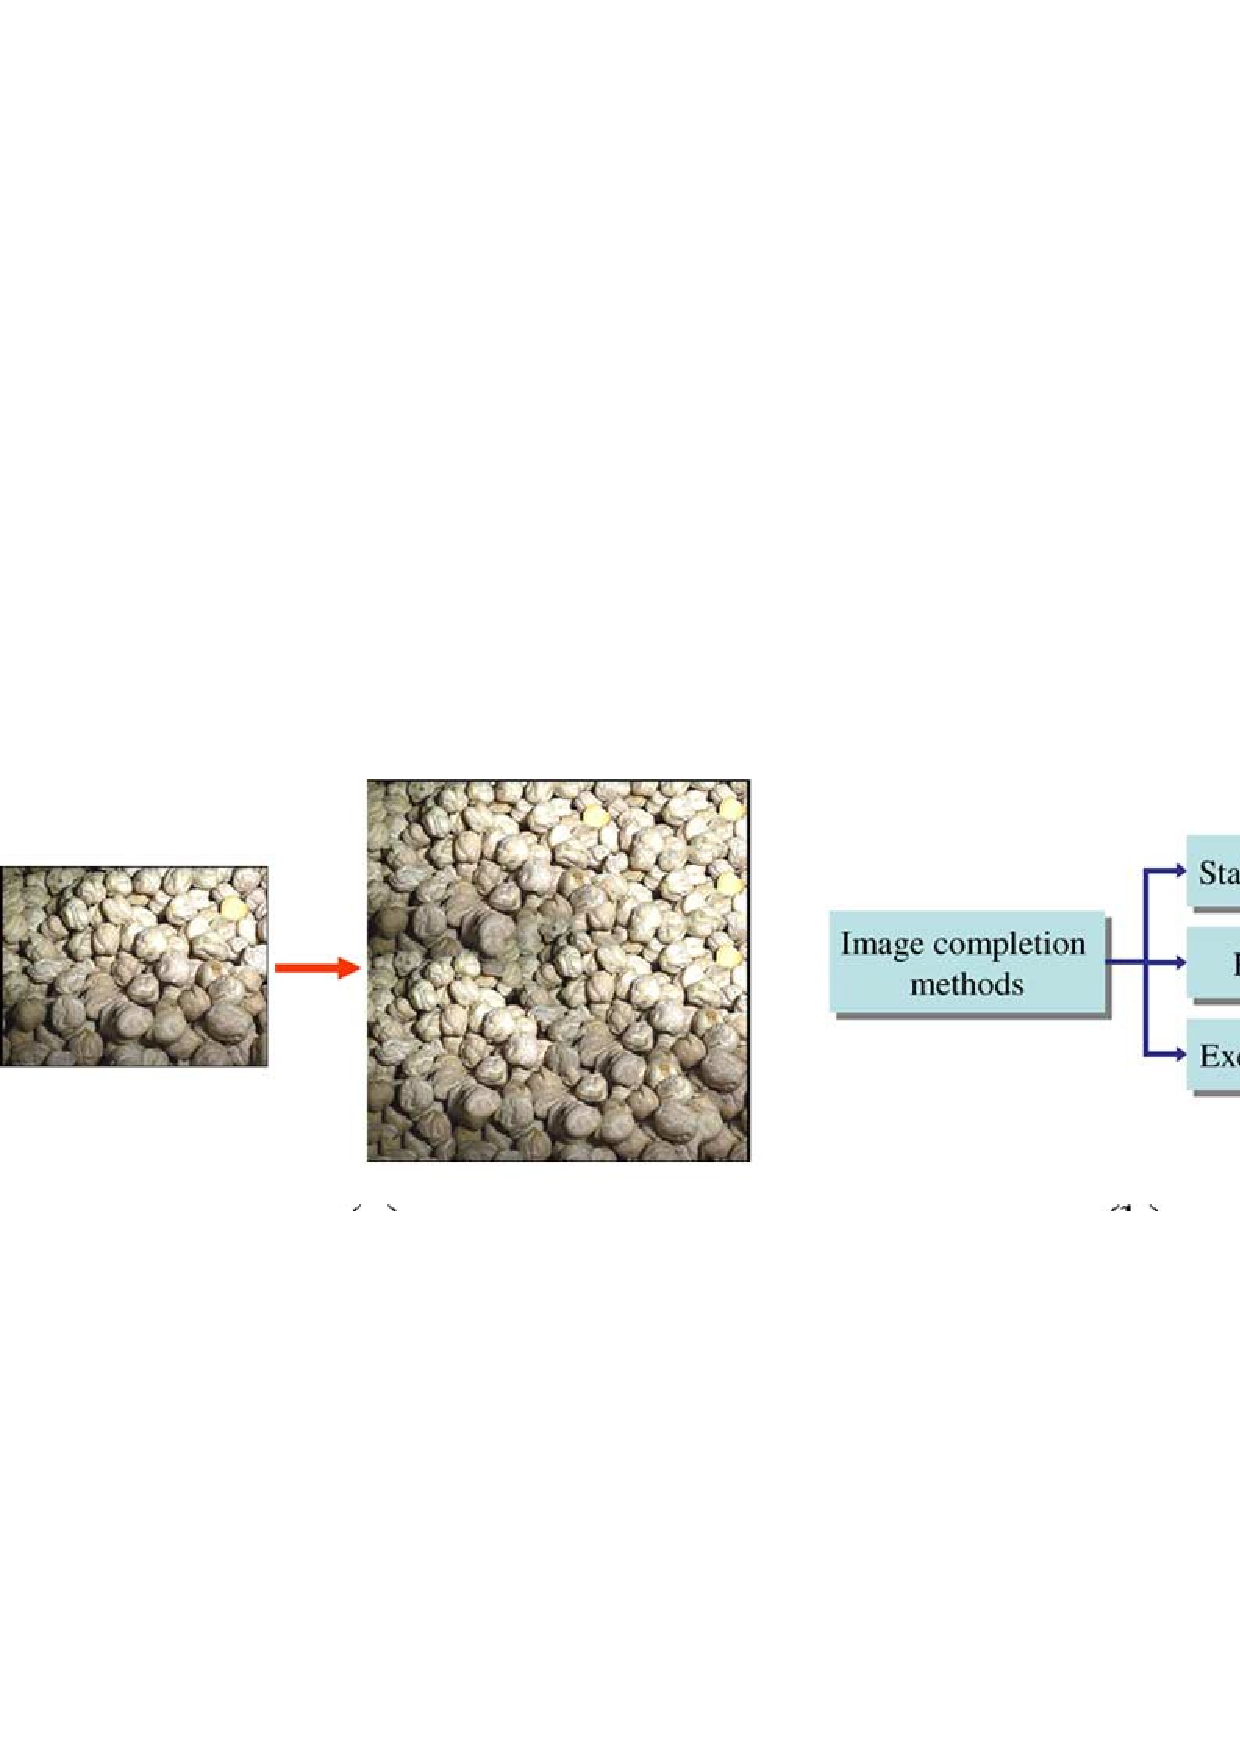
\includegraphics[width=4in]{prune2.pdf}\\
  \caption{Image Completion}\label{}
\end{figure}
\end{frame}


\begin{frame}
\frametitle{\textbf{4.Image Completion Using Efficient Belief Propagation
Via Priority Scheduling and Dynamic Pruning}}
\begin{itemize}
\item Exemplar-based techniques  fill the unknown region simply by copying content from the observed part of the image.
\item All exemplar-based techniques for texture synthesis  were either pixel-based or patch-based, meaning that the final texture was synthesized one pixel, or one patch at a time
\item A new exemplar-based framework  which treats image completion, texture synthesis, and image inpainting in a unified manner.
\item All   image-editing tasks in the form of a discrete global optimization which is used to avoid visually inconsistent results.
\end{itemize}
\end{frame}

\begin{frame}
\frametitle{\textbf{4.Image Completion Using Efficient Belief Propagation
Via Priority Scheduling and Dynamic Pruning}}
\begin{itemize}
\item Novel optimization scheme, called priority belief propagation (BP) is used  which carries two very important extensions over the standard BP algorithm
\begin{enumerate}
  \item \textbf{Priority-based message scheduling}
  \item \textbf{Dynamic label pruning}
\end{enumerate}
\item As one of  major limitation of the BP algorithm  is  its inefficiency in handling MRFs with very large discrete state spaces is considered to resolve by these extension techniques.
\end{itemize}
\end{frame}


\begin{frame}
\frametitle{\textbf{4.Image Completion Using Efficient Belief Propagation
Via Priority Scheduling and Dynamic Pruning}}
\begin{itemize}
\item Priority Belief Propagation  can be used for other types of completion problems such as video completion or geometric completion,constrained texture synthesis
\item Priority-BP algorithm, which is a generic MRF optimization scheme can be used to other labeling problems also.
\end{itemize}
\end{frame}


\begin{frame}
\frametitle{\textbf{5.Low Memory Cost Block-Based Belief Propagation For Stereo Correspondence}}
\begin{itemize}
\item Stereo correspondence is used in computer vision to find the depth among the cameras and objects.
\item The depth inference problem could be further transformed  to  a disparity inference problem by assuming that the cameras and objects are under epipolar geometry.
\item The inferred disparity information could be widely applied to tracking, surveillance system, and multiview video coding.
\end{itemize}
\end{frame}


\begin{frame}
\frametitle{\textbf{5.Low Memory Cost Block-Based Belief Propagation For Stereo Correspondence}}
The stereo matching algorithms can be roughly divided into two categories.
\begin{enumerate}
  \item \textbf{Local approaches}
  \item \textbf{Global approaches}
\end{enumerate}
\end{frame}

\begin{frame}
\frametitle{\textbf{5.Low Memory Cost Block-Based Belief Propagation For Stereo Correspondence}}
\begin{itemize}
\item Local approaches select disparities of image pixels using the information in a window. Therefore local approaches are faster than global approaches.
\item  It results in poor accuracy since the local approaches could not deal with textureless regions and occluded regions well due to the insufficient information in window.
\item On the other hand, global approaches can handle the textureless and occluded regions well by formulating disparity inference as an energy minimization problem
\end{itemize}
\end{frame}
\begin{frame}
\begin{figure}
  % Requires \usepackage{graphicx}
  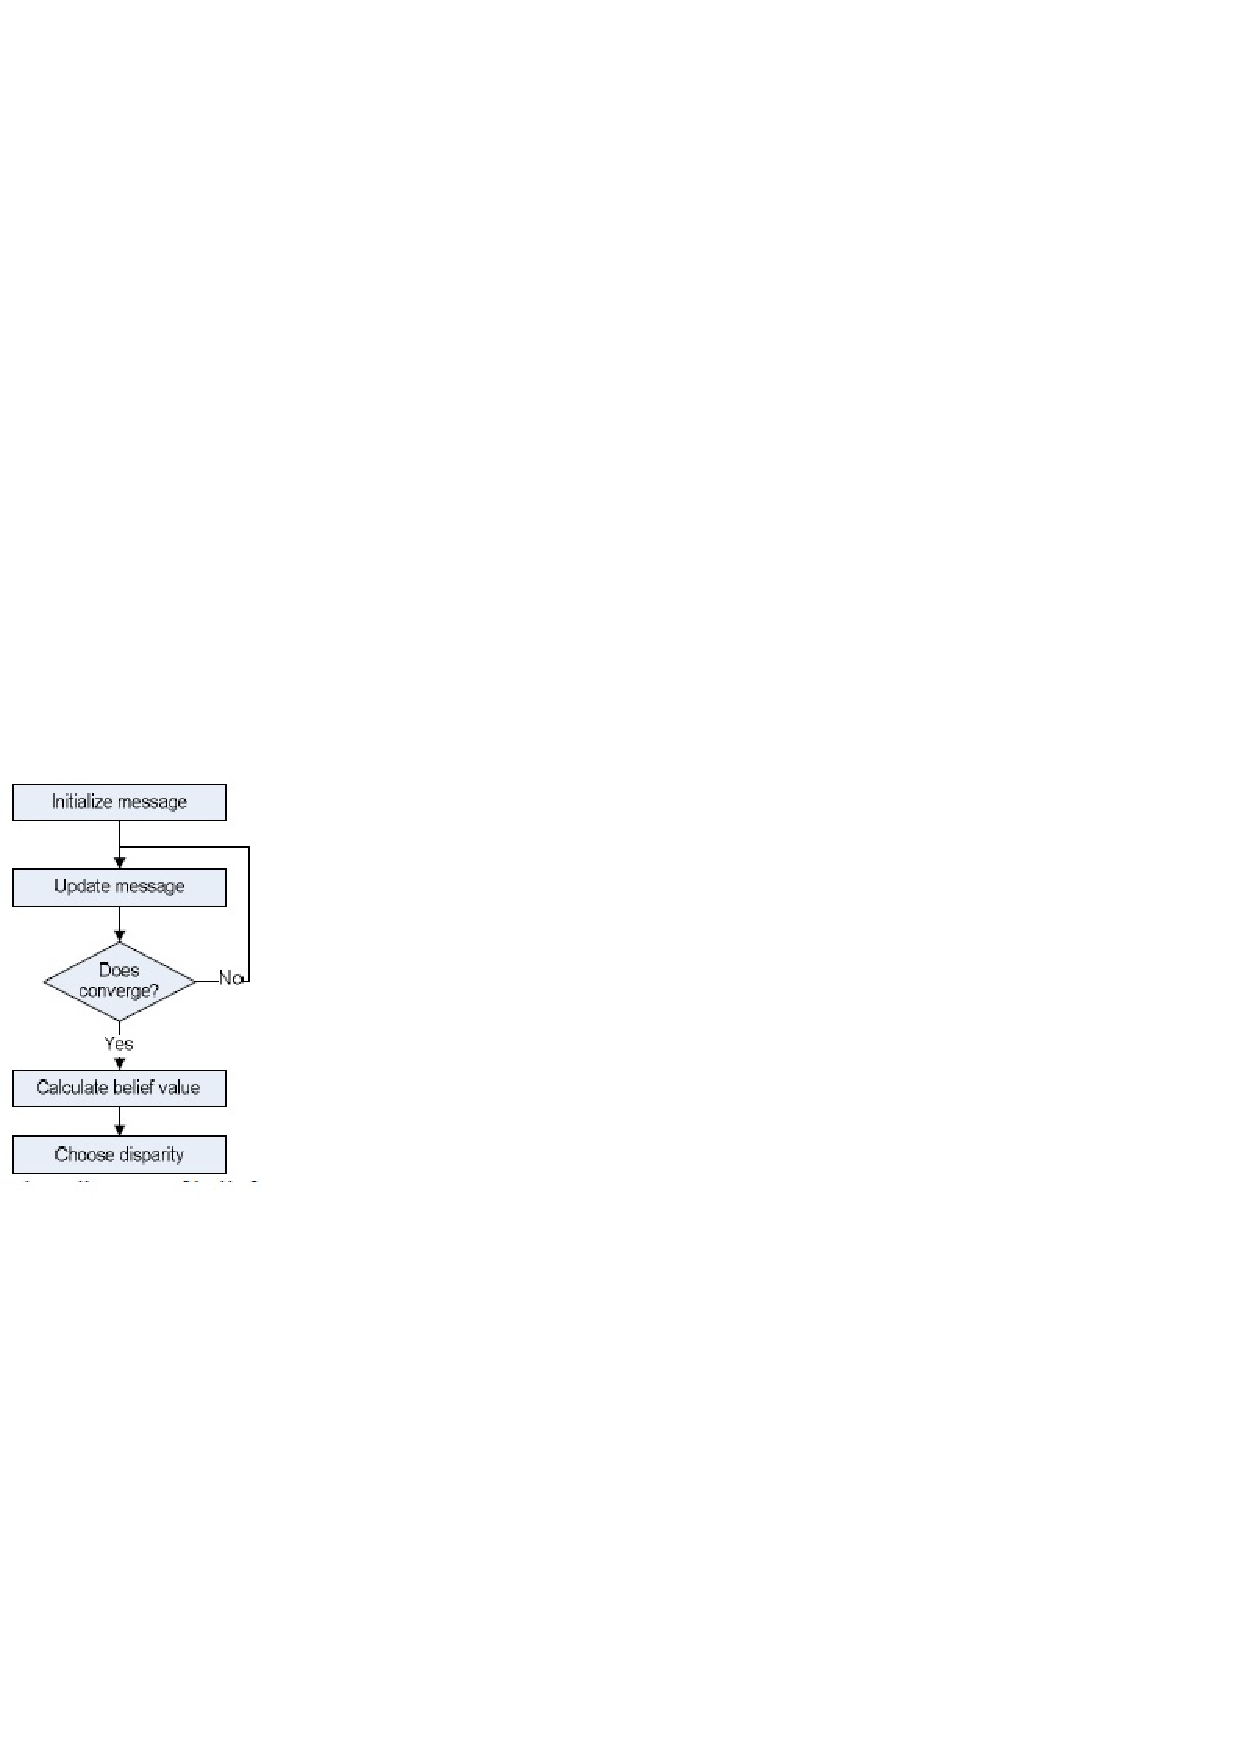
\includegraphics[width=1in]{block1.pdf}\\
  \caption{Flow diagram of Belief Propagation}\label{}
\end{figure}
\end{frame}

\begin{frame}
\frametitle{\textbf{5.Low Memory Cost Block-Based Belief Propagation For Stereo Correspondence}}
\begin{itemize}
\item The BP algorithms construct 2-D graph structures with nodes representing all the pixels in the disparity images to find the disparity map with energy closer to the global minima
\item The vast number of nodes in the 2-D graph  result in  extremely high computation complexity, thereby rendering 2-D optimization is too difficult to be directly implemented for real-time application.
\item A block-based BP algorithm that directly partitions an image into separated independent blocks. Thus, can reduce the memory size significantly due to block based computation.
 \item The independent blocks also enable parallel computation by multiple computation units. Moreover earlier convergence for each block can also improve the long running time.
\end{itemize}
\end{frame}
\begin{frame}
\begin{figure}
   %Requires \usepackage{graphicx}
 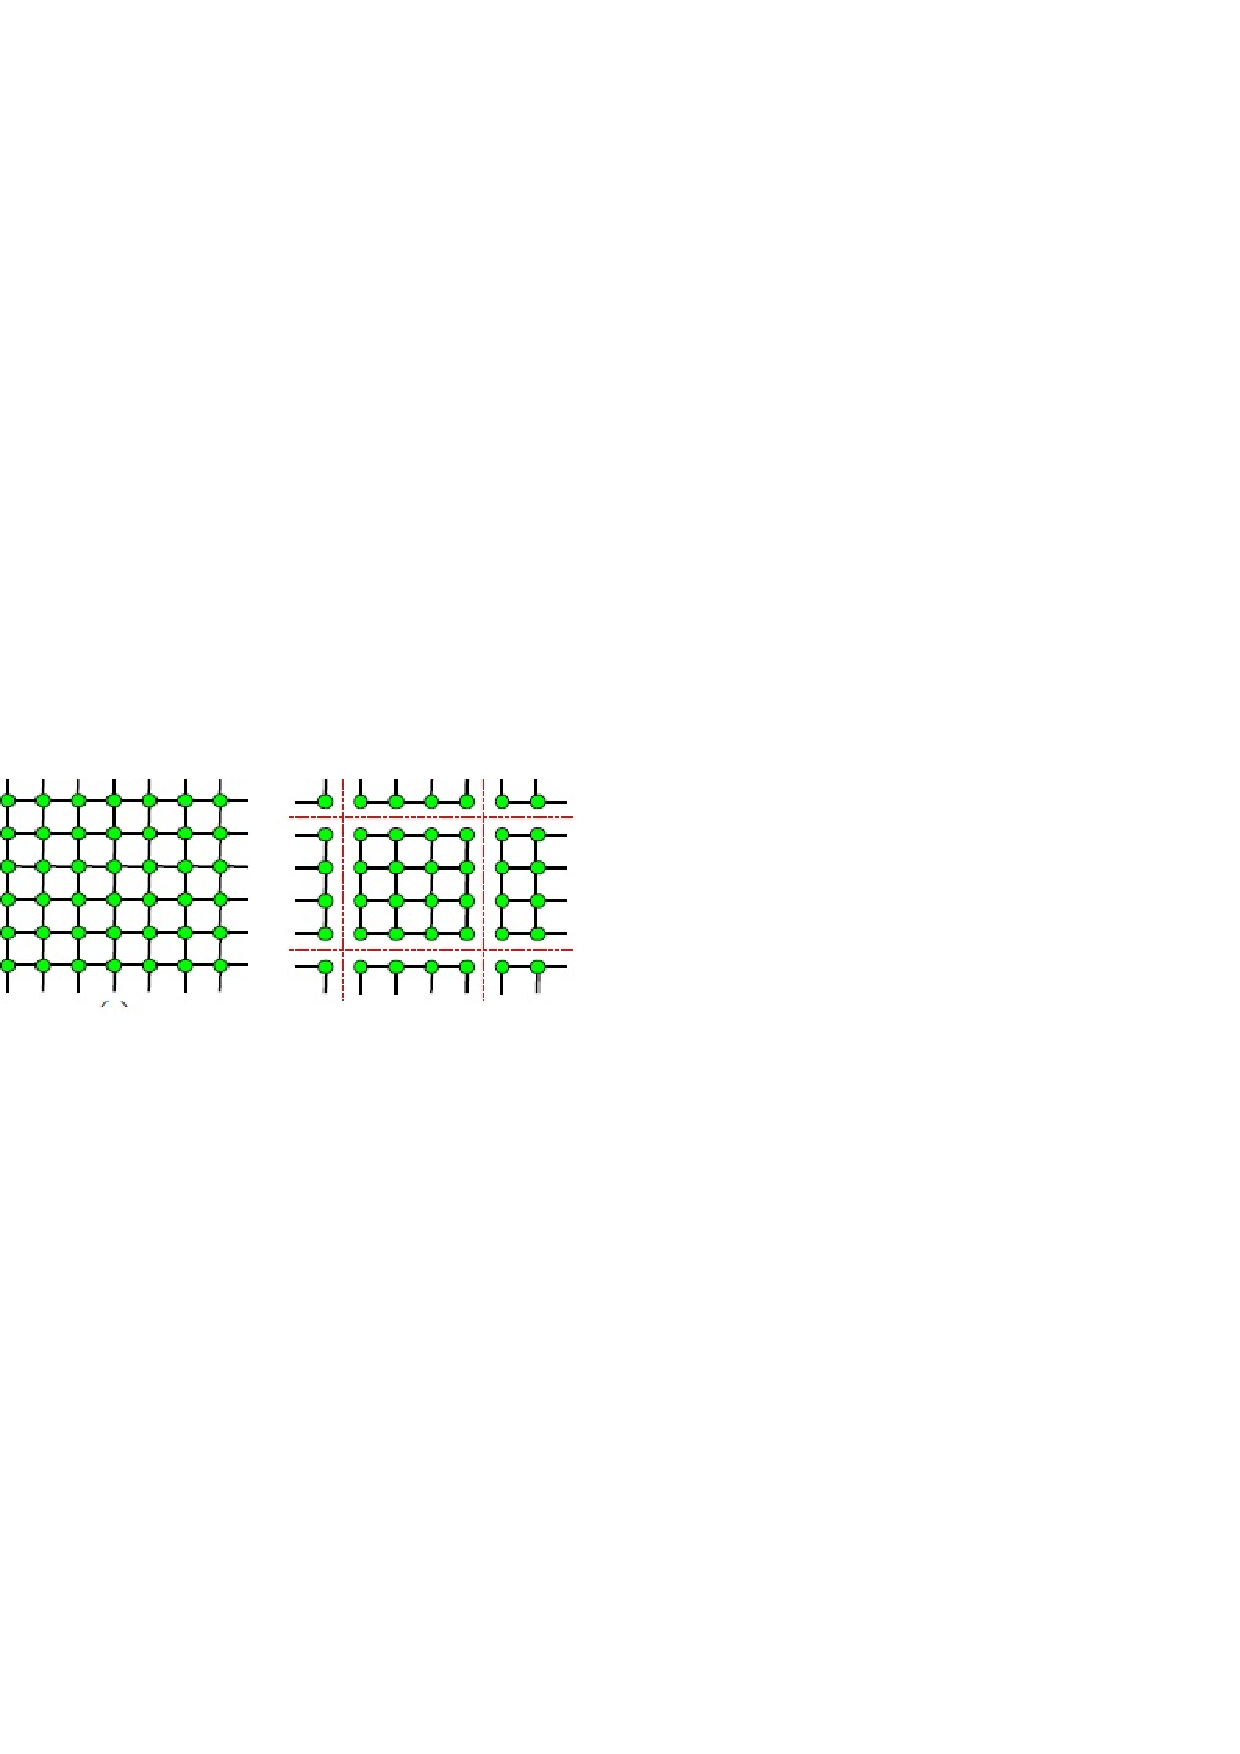
\includegraphics[width=4in]{block2.pdf}\\
  \caption{Graph of typical and block based BP}\label{}
2D Graph Model
\end{figure}
\end{frame}


\begin{frame}
\frametitle{\textbf{5.Low Memory Cost Block-Based Belief Propagation For Stereo Correspondence}}
\textbf{Results}
\begin{itemize}
\item A new stereo matching algorithm partitions an image to block and optimizes with belief propagation technique.This method reduces memory storage size by 99 percentage
with good performance.
\item To enhance the interaction  between neighboring blocks such that the independent block could extract useful information from  neighboring finished processing blocks are possible with block belief propagation.
\end{itemize}
\end{frame}

\begin{frame}
\frametitle{\textbf{6.Task Parallel Implementation Of Belief Propagation in Factor Graphs}}
\begin{itemize}
\item Graphical models are essential tools for probabilistic reasoning. Factor graphs  are  emerged as a unified model of directed graphs (e.g. Bayesian networks) and undirected graphs (e.g. Markov networks).
\item  A factor graph  represents a joint probability distribution ie.written as a product of factors, each involving a subset of random variables.
\item Factor graphs have found applications in   Image processing,Bioinformatics and  Error-control decoding used in digital communications.\\
\end{itemize}
\end{frame}


\begin{frame}
\frametitle{\textbf{6.Task Parallel Implementation Of Belief Propagation In Factor Graphs}}
\textbf{Relation between  Factor graphs and Belief Propagation.}
\begin{itemize}
  \item Inference is a problem of computing posterior probability distribution of certain variables given some value as observed or evidence variables.
  \item In factor graphs, inference proceeds with the belief propagation algorithm .
  \item Belief propagation is a process of passing messages along the edges of a graph.
  \item Processing each message requires a set of operations with respect to the probability distribution of the random variables in a graph.
  \item Such distribution is represented by potential tables.
  \item The complexity of belief propagation increases dramatically as the number of states of variables and node degrees of a graph increase.
\end{itemize}
\end{frame}

\begin{frame}
\frametitle{\textbf{6.Task Parallel Implementation Of Belief Propagation in Factor Graphs}}
\textbf{Results}
\begin{itemize}
\item Belief propagation must be performed in real time.Many parallel techniques have been proposed for belief propagation in factor graphs.
\item Parallelizing belief propagation in acyclic factor graphs still remains a challenging problem due to the precedence constraints among the nodes in the graphs.
\item Task scheduling is used in parallel computing is an efficient tool  for linear algebra problem on general-purpose multi-core processors.
\item The  methods used for implementation of Belief Propagation using factor graphs are task dependency graph  by using a dynamic task scheduler.
\end{itemize}
\end{frame}

\begin{frame}
\frametitle{\textbf{7.Hardware-Efficient Belief Propagation}}
\begin{itemize}
\item The success of BP is due to its regularity and simplicity.
\item It uses a simple message update process to iteratively refine the beliefs of labels for each node.
\item A message sent from one node to another is updated according to neighboring messages and local energy functions.
\item Loopy belief  propagation (BP)is an effective solution for assigning labels to the nodes of a graphical model such as the Markov random field (MRF).
\end{itemize}
\end{frame}

\begin{frame}
\frametitle{\textbf{7.Hardware-Efficient Belief Propagation}}
\begin{itemize}
\item BP algorithms generally require a great amount of memory for storing the messages, typically on the order of tens to hundreds times larger than the input data.
\item Since each message is processed hundreds of times, the saving/loading of  messages consumes considerable bandwidth.
\item Although BP may work on high-end platforms such as desktops, it cannot be applied to most consumer electronic devices that have limited memory, computational power, and energy.
\item It is  difficult to  utilize  hardware  parallelism  to accelerate BP
\end{itemize}
\end{frame}

\begin{frame}
\frametitle{\textbf{7.Hardware-Efficient Belief Propagation}}
The two techniques are used for sequential procedure to accelerate BP
\begin{itemize}
\item The first one is tile-based BP  splits the Markov random field (MRF) into many tiles and only stores the messages across the neighboring tiles. The memory and bandwidth required by this technique is only a fraction of the ordinary BP algorithms.

\item Second technique is that  fast message construction technique is based on the observation that many hypotheses used to construct the mesasages are repetitive.therefore, they only need to be computed once which reduces running time of the  alogorithm

\end{itemize}
\end{frame}

\begin{frame}
\frametitle{\textbf{7.Hardware-Efficient Belief Propagation}}
\textbf{Results}
\begin{itemize}
\item These techniques can be realized in both hardware and software.
\item A software reference implementation compatible to  the  Middlebury  MRF  library which  is  available  online.
\item  First  hardware  is a very large scale integration (VLSI) circuit and the second one a graphic processing unit (GPU) program are analyzed
\item \textbf{ A tile-based message passing and fast message construction  algorithm }greatly reduced the memory, bandwidth, and computational costs of BP and enabled the parallel processing. With these two techniques  BP  can be  more suitable for low-cost and power limited consumer electronics.
\end{itemize}
\end{frame}

\begin{frame}
\frametitle{\textbf{8.PMBP: PatchMatch Belief Propagation for Correspondence Field Estimation}}
Patch Match is a simple, yet very powerful and successful method for optimizing Continuous labelling problems.
The two main approaches  used are
\begin{itemize}
\item The update of the solution space by sampling
\item The use of the spatial neighborhood to propagate samples.
\end{itemize}
These approaches are related to steps in a specific form of belief Propagation in the continuous space, called Particle Belief Propagation (PBP)
\end{frame}

\begin{frame}
\frametitle{\textbf{8.PMBP: PatchMatch Belief Propagation for Correspondence Field Estimation}}
\begin{itemize}
\item The two approaches used in this research yields a new algorithm called Patch Match Belief Propagation for Correspondence Field estimation (PMBP),which is more accurate than Patch Match and orders of magnitude faster than PBP.
\item The link between the popular PatchMatch method and the very well-known Belief propagation algorithm.
\item These approaches  can be  used as both in terms of applications, such as optical flow, as well as algorithms such as different forms of message passing e.g.  Treereweighted
\end{itemize}
\end{frame}

\begin{frame}
\frametitle{\textbf{9.Learning continuous time Bayesian network classifiers}}

\begin{itemize}
\item Continuous time Bayesian network classifiers are designed for analyzing multivariate streaming data when time duration of event matters.
\item The  continuous time  Bayesian network  classifiers are  considered  in  the  case where  complete  data is available.
\item Conditional log-likelihood  scoring is developed for structural learning on continuous time Bayesian network classifiers.
\item Results show that conditional  log-likelihood  scoring combined with Bayesian parameter estimation outperforms marginal log-likelihood scoring.\item Conditional log-likelihood  scoring becomes even more effective when  the amount of available data is limited.
\end{itemize}
\end{frame}

\begin{frame}
\frametitle{\textbf{9.Learning continuous time Bayesian network classifiers}}
\begin{itemize}
\item Conditional log-likelihood scoring function is used  to learn continuous time Bayesian network classifiers from multivariate streaming  data.
\item Same function can be used for classifying multivariate trajectories in the case where the class is static .
\item The quality of the classification performances also suggests to extend the Continuous Time Bayesian Network Classifiers to the clustering problem.
\end{itemize}
\end{frame}

\begin{frame}
\frametitle{\textbf{Conclusion}}
\begin{itemize}
\item The graphical representation or models for multidimentional probability distributions such as Markov  Random Fields and  Bayesian Networks are used for Belief Propagation Techniques.

\item  Some of the applications to optimize Markov  Random Fields to speed up the  Belief Propagation  are used for face recognition, for image completion and low level vision problem,
\item To reduce memory size and computation time block based Belief Propagation algorithm ,tile based Belief Propagation and fast construction techniques are used.
\end{itemize}
\end{frame}







\begin{frame}
\frametitle{References1}
\begin{enumerate}
\item Judea Pearl, \textbf{Probabilistic Reasoning in Intelligent Systems},
Kaufmann Morgann Publishers, Second Revised And updated Edition,San Francisco, California, 1998.
\item Yu-Chang And Nelson Chang,\textbf{Low Memory Cost Block-Based Belief Propagation For Stereo Correspondence},
1-4244-1017-7187,IEEE Transisition
\item F.Besse,C.Rother,A.Fitzgibbon,J.Kautz
\textbf{Pmbp:Patchmatch Belief Propagation For Correspondence Field Estimation},
University College Of London U.K.,Microsoft Research Cambridge ,2012
\item Nam Ma,Yinglong Xia,Viktorprasanna
\textbf{Task Parallel Implementation Of Belief Propagation In Factor Graphs}
This Research Was Suppored By U.S.National Foundation Under Grant No.Cns-101880
\end{enumerate}
\end{frame}
\begin{frame}
\frametitle{References2}
\begin{enumerate}
\item Wonjun Hwang Kyungshik,Roh Junmo Kim
\textbf{Markov Network-Based Unified Classifier For Face Identification}
This ICCV 2013 Paper is Open Access Available In IEEE Xplore
\item Radu Timofte,Lucvan Gool
\textbf{Efficient Loopy Belief Propagation Using The Four Color Theorem}
Isics,Esat-Psi/Iminds V,Belgium,Computer Vision Lab,Zurich,Switzerland
\item Nikos Komadakis,Georgios Tziritas
\textbf{Image Completion Using Efficient Belief Propagation Via Priority Scheduling And Dynamic Pruning}
IEEE Transactions In Image Processing ,Volume;16,No.11,November 2007
\end{enumerate}
\end{frame}
\begin{frame}
\frametitle{References3}
\begin{enumerate}
\item Chia-Kai Liang,Chao-Chung Cheng,Yen-Cheieh Lai
\textbf{Hardware-Efficient Belief Propagation}
IEEE Transactions On Circuits And Systems For Video Technology Vol;21,No.5,May 2011
\item Daniele Codecasa,Fabiostella
\textbf{Learning Continuous Time Bayesian Network Classifiers}
International Journal Of Approximate Reasoning,55(2014) 1728-1746
\item Pedro F.Felzenszwalb,Daniel P.Huttenlocher
\textbf{Efficient Belief Propagation For Early Vision}
International Journal Of Computer Vision (Springer Science)70(1),41-54,2006
\item Jianguo Ding
\textbf{Probabilistic Inferences In Bayesian Networks}
International Journal Of Computer Science,Arxiv:1011.0935V2,5 November 2010
\end{enumerate}
\end{frame}








%Slide which includes last slides
\begin{frame}
\centerline{\textbf{\begin{Huge}Thank You...\end{Huge}}}
\end{frame}

\end{document}

